\documentclass[a4paper]{article}
\usepackage{amsmath,amssymb,amsthm}
\usepackage{txfonts} %% per \fint
\usepackage{graphicx}
\usepackage{natbib} %% per modificare bibliography

\title{INdAM Workshop on vector-valued mappings
  and systems of PDE's}
\date{Roma, May 17-21 2010}

\newcommand{\separatore}{\bigskip\hrule\bigskip}
\newcommand{\titolo}[1]{\bigskip\pagebreak[3]\noindent{\large\bf #1}\\\nopagebreak[4]}
\newcommand{\autore}[1]{{\bf #1}\\\nopagebreak[4]}
\newcommand{\email}[1]{(#1)\\ \nopagebreak[4]\smallskip }
\newcommand{\medint}{\fint}
\newcommand{\rn}{\mathbb R^n}
\newcommand{\D}{\nabla}
\newcommand{\lio}{L^\infty(\Omega)}
\newcommand{\lip}{W^{1,\infty}(\Omega)}
\newcommand{\R}{\mathbb R}
\newcommand{\dx}{dx}

\newcommand{\buh}[1]{\textsf{#1}\\}
\DeclareMathOperator{\dive}{div}
\renewcommand{\div}{\dive}

%\renewcommand{\bibsection}{\bigskip{\noindent\bf References}\\\nopagebreak[4]}
\renewcommand{\bibsection}{}

\def\elle#1{L^{#1}(\Omega)}
\def\norma#1#2{\|#1\|_{\lower 4pt \hbox{$\scriptstyle #2$}}}

\begin{document}
\thispagestyle{empty}
\vspace{2cm}
\begin{center}
  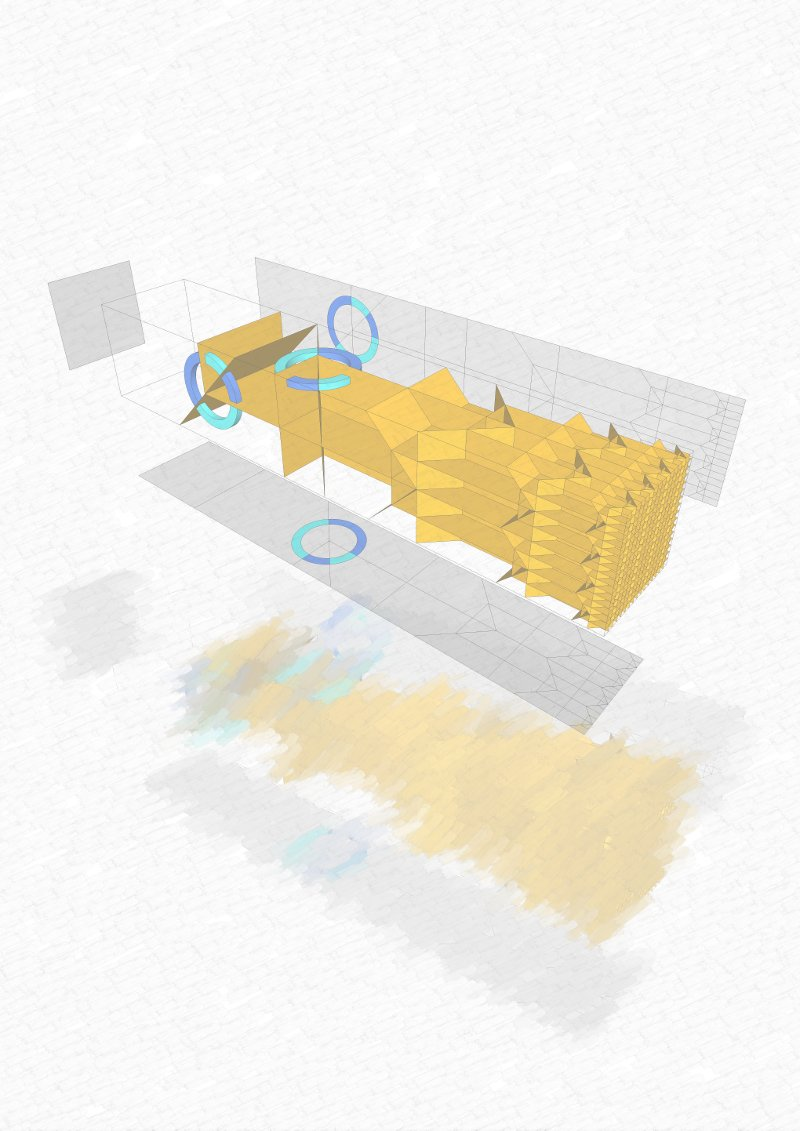
\includegraphics[width=\textwidth]{bg.jpg}
  \vspace{-19cm}

  \Huge
  \buh{Incontro \rm\raisebox{5pt}{<}$\mathbb N\delta$A\rule{1pt}{0pt}\raisebox{0.7em}{\rotatebox{270}{$\Sigma$}}}
  \large
  \buh{Istituto Nazionale di Alta Matematica}
  \bigskip
  \bf
  \Huge
  \buh{Workshop on Vector-Valued Mappings}
  \Huge
  \buh{and Systems of PDE's}
  \huge
  \buh{}
  \huge
  % \vspace{1cm}
  \bigskip
  \Large
  \buh{\Huge\textbf{ROMA}}
  \buh{May 17--21, 2010}
  \buh{INdAM, Istituto Nazionale di Alta Matematica,}
  \buh{Citt\`a Universitaria
    P.le A. Moro n.~5}
  \vspace{1.5cm}
  \buh{}%\Huge\textbf{ABSTRACTS}}

  \vspace{1.5cm}
  \Large
  \buh{Invited Speakers:}
  \medskip
  \small
  \begin{tabular}{rlcrlcrl}
    Micol& Amar &\mbox{}\ \mbox{}& 
    Kari &Astala &\mbox{}\ \mbox{}& 
    Michael &Bildhauer\\
    % 
    Lucio &Boccardo && 
    Arrigo & Cellina &&
    Giovanni & Cupini\\
    % 
    Bernard & Dacorogna &&
    Frank & Duzaar &&
    Matteo & Focardi \\
    % 
    Irene & Fonseca &&
    Flavia & Giannetti &&
    Luigi & Greco \\
    % 
    Stanislav & Hencl &&
    Tadeusz & Iwaniec &&
    Olivier & Kneuss \\
    % 
    Tommaso & Leonori &&
    Francesco & Maggi &&
    Carlo & Mariconda \\
    % 
    Elvira & Mascolo &&
    Giuseppe & Mingione &&
    Gioconda & Moscariello \\
    % 
    Carlo & Nitsch &&
    Luigi & Orsina &&
    Emanuele & Paolini \\
    % 
    Antonia & Passarelli di Napoli\hspace{-1.0cm}\mbox{}&&
    Aldo & Pratelli &&
    Giulia & Treu \\
    & &&
    Anna & Verde 
  \end{tabular}\\
  \bigskip
  \Large
  \buh{Organizers:}
  \small
  \begin{tabular}{rlcl}
    Paolo & Marcellini &\mbox{}\ \mbox{}&{Universit\`a di Firenze}\hspace{-3cm}\mbox{}\\
    Carlo & Sbordone &&{Universit\`a di Napoli}\\
  \end{tabular}\\
  \vspace{1cm}
  \bigskip
  \Large
  % \buh{Contact:}
  \small
  \bf\textsf{http://www.math.unif{}i.it/users/cdvedp/eventi/indam10/}
  % \verb|http://www.math.unifi.it/~cdvedp/indam/|
  \hspace{1cm}
  \bf\textsf{indam10@math.unif{}i.it}
  % \verb|indam07@math.unifi.it|

\end{center}
\newpage
\maketitle

\centerline{\Large \bf ABSTRACTS}

\bigskip

\titolo{Homogenization of chessboard structures}%
\autore{Micol Amar}%
\email{amar@dmmm.uniroma1.it}%

\noindent
We study the geodesics in a planar chessboard structure.
The results for a fixed structure allow
us to infer the properties of the Finsler metrics obtained, with a homogenization
procedure, as limits of oscillating chessboard structures.


\separatore  \titolo{Sharp bounds for quasiconformal mappings in the critical $W^{1,p}$-space}%
\autore{Kari Astala}%
\email{astala@mappi.helsinki.fi}%

\noindent
\sloppypar
In two dimensions it is known that $K$-quasiconformal mappings have
locally $L^p$-integrable derivatives for every $p < 2K/(K-1)$, and this
yields similar Sobolev-regularity for solutions to elliptic PDE's.
Basic examples show that integrability does not hold at $p = 2K/(K-1)$.

In this talk, based on joint work with Iwaniec, Prause and Saksman, I
will discuss if something can be said at the critical exponent $p =
2K/(K-1)$:  Are the $K$-quasiconformal derivatives in some weighted
$L^p$-space?

The question is closely related to understanding the well-known
Burkholder functional, a rank-one convex functional which is expected
to be quasiconvex. Thus the talk can also be considered as a
discussion on quasiconformal methods towards understanding the
Burkholder functional. 

\separatore  \titolo{On local generalized minimizers and local stress tensors for variational problems with linear growth}%
\autore{Michael Bildhauer}%
\email{bibi@math.uni-sb.de}%

\noindent \emph{joint work with Darya Apushkinskaya and Martin Fuchs}\\

\noindent
Uniqueness and regularity results for local vector-valued
generalized minimizers and for local stress tensors associated to
variational problems with linear growth conditions are established.
Assuming that the energy density $f$ has the structure $f(Z) = h(|Z|)$,
only very weak ellipticity assumptions are required. For the proof
we combine arguments from measure theory and convex analysis with some
recent regularity results.


\separatore  \titolo{Dirichlet problems with singular convection terms and applications to some systems}%
\autore{Lucio Boccardo}%
\email{boccardo@mat.uniroma1.it}%

\noindent
Let $\Omega$ be a bounded, open subset of $\R^N$, $N > 2$  and $M :\Omega \to \R^{N^2}$,
 be a bounded and measurable matrix such that
$$
 \alpha |\xi|^2\leq
  M(x)\xi\cdot\xi, \quad |M(x)| \leq\beta,  \quad  \mbox{a.e.}\; x\in\Omega,\quad \forall \;\xi\in\R^N\,.
$$
Under the assumptions    $|E|\in\elle N$, $f\in\elle{m}$ ($m\geq\frac{2N}{N+2}$) and $\mu>0$
 large enough,
Guido Stampacchia proved that the boundary value problem

$$ \mbox{$-\div(M(x)\nabla u -u\,E(x)) + \mu u=f(x)$ in $\Omega$}, \quad
 \mbox{$u =0$ on $\partial\Omega$} 
 $$
 has a unique weak  solution $u$ with some summability properties.


If $\mu=0$, it is possible to prove the coercivity  of the differential operator only if
$\|{E}\|_{L^{N}(\Omega)}$ is small enough; nevertheless, if $f\in\elle m$,  $m\geq1 $,
existence and summability properties (depending on $m$, but independent of the size of
$\norma{E}{}$)  of weak or distributional solutions were recently proved by the
author.

We present examples of explicit radial solutions which show how existence and
summability results can be lost in the borderline cases when $f$ and $E$ are smooth enough
but instead of the inclusion $E\in (\elle N)^{N}$ the weaker condition $E\in (\elle q)^{N}$
for any $q<N$ is fullfilled;
in general, if $|E|\leq\frac{\,A\,}{|x| }$, $A>0$, and $0\in\Omega$, we prove existence and
summability properties of the solutions, depending on $m$ and on the size of the constant
$A$. 

One of the main points of the talk concerns equations with  $E\in(L^{2} (\Omega))^{N}$.
The starting point here is the definition of solution since the distributional definition does
not work. It is possible to give meaning to the solution thanks to the concept of {\sl
entropy solutions}.

Then we discuss some existence results about the system
($0<\theta<1$)
$$ 
{\left\{
\begin{array}{ll}
\displaystyle
-\div(M_0(x)\nabla u)+u= 
-\div(u\,M(x)\nabla z)+f 
(x)
 & \mbox{in $\Omega$,} 
 \\
 \displaystyle
-\div (M(x)\nabla z 
 )={u^\theta}
  & \mbox{in $\Omega$,} \\
 u=z=0 & \mbox{on $\partial\Omega$.}   \\
\end{array}
\right.}
$$


\separatore  \titolo{tba}%
\autore{Arrigo Cellina}%
\email{arrigo.cellina@unimib.it}%

\separatore  \titolo{Regularity of minimizers under sharp anisotropic general growth conditions}%
\autore{Giovanni Cupini}%
\email{cupini@dm.unibo.it}%

\noindent
In some recent papers by Lieberman and Bildhauer-Fuchs the regularity of
minimizers of energy-functionals is studied assuming a priori that they are
bounded. In a joint paper with P.Marcellini and E.Mascolo we prove the local
boundedness of minimizers for functionals with non-homogeneous densities
satisfying anisotropic general growth conditions. As a consequence of
the above cited papers we obtain the local Lipschitz-continuity of minimizers
under sharp assumptions on the exponents of anisotropic growth.

\separatore  \titolo{On the pullback equation and Darboux theorem}%
\autore{Bernard Dacorogna}%
\email{bernard.dacorogna@epfl.ch}%

\noindent
We discuss the existence of a diffeomorphism $\varphi:\mathbb{R}%
^{n}\rightarrow\mathbb{R}^{n}$ verifying
\[
\varphi^{\ast}\left(  g\right)  =f
\]
where $f,g$ are closed differential $2-$forms. Componentwise the equation
reads as%
\[
\sum_{1\leq i<j\leq n}g_{ij}\left(  \varphi\left(  x\right)  \right)
d\varphi^{i}\wedge d\varphi^{j}=\sum_{1\leq i<j\leq n}f_{ij}\left(  x\right)
dx^{i}\wedge dx^{j}\,.
\]

1) We generalize the celebrated Darboux theorem in two directions. First we
obtain optimal regularity in H\"{o}lder spaces for the local problem and then,
under some necessary additional hypotheses, we get global existence as well as
regularity. We thus extend to $2-$forms the results of Moser and
Dacorogna-Moser obtained for the case of volume forms $k=n.\smallskip$

2) We will say few words on the more difficult problem of $k-$forms, when
$3\leq k\leq n-1.$\bigskip

[1] Bandyopadhyay S. and Dacorogna B., On the pullback equation $\varphi
^{\ast}\left(  g\right)  =f,$ \textit{Ann. Inst. Henri Poincar\'{e}, Analyse
  Non Lin\'{e}aire},\textit{ }\textbf{26} (2009), 1717-1741.$\smallskip$

[2] Bandyopadhyay S., Dacorogna B. and Kneuss O., The pullback equation for
degenerate forms,  \textit{Disc. Cont. Dyn. Syst. Series A}, \textbf{27}
(2010), 657-691.$\smallskip$

[3] Dacorogna B. and Kneuss O., Divisibility in Grassmann algebra, in preparation.

\separatore  \titolo{Regularity for parabolic systems with degenerate diffusion}%
\autore{Frank Duzaar}%
\email{duzaar@mi.uni-erlangen.de}%

\noindent
The aim of the talk is twofold. On one hand we want to present a new technique called $p$-caloric approximation, which is a proper generalization of the classical compactness methods first developed by DeGiorgi with his Harmonic Approximation Lemma. This last result, initially introduced in the setting of Geometric Measure Theory to prove the regularity of minimal surfaces, is nowadays a classical tool to prove linearization and regularity results for vectorial problems. Here we develop a very far reaching version of this general principle devised to linearize general degenerate parabolic systems. The use of this result in turn allows to achieve the subsequent and main aim of the paper, that is the implementation of a partial regularity theory for parabolic systems with degenerate diffusion of the type
\begin{equation}
\label{qds-1}
\partial_t u - \dive a(Du)=0\,,
\end{equation}
without necessarily assuming a quasi-diagonal structure, i.e. a structure prescribing that the gradient non-linearities depend only on the explicit scalar quantity $|Du|$. Indeed, the by now classical theory of DiBenedetto  introduces the fundamental concept of intrinsic geometry and allows to deal with the classical degenerate parabolic $p$-Laplacean system
\begin{equation}
\label{qds0}
\partial_t u - \dive (|Du|^{p-2}Du)=0
\end{equation}
and more general with systems of the type
\begin{equation}
\label{qds}
\partial_t u - \dive \big(g(|Du|)Du\big)=0\,.
\end{equation}
Here, we take such regularity results as a starting point and develop
a partial regularity theory -- regularity of solutions outside a
negligible closed subset of the domain -- applying to general
degenerate parabolic systems of the type \eqref{qds-1}, thereby not
necessarily satisfying a structure assumption as \eqref{qds}. The
partial regularity rather than the everywhere one, is natural since
even in the non-degenerate case, when considering systems with general
structure, singularities may occur. The proof of the almost everywhere
regularity of solutions is then achieved via an extremely delicate
combination of local linearization methods, together with a proper use
of DiBenedetto's intrinsic geometry: the general approach that
consists in performing the local analysis by considering parabolic
cylinders whose space-time scaling depend on the local behavior of the
solution itself. The combination of these approaches was exactly the
missing link to prove partial regularity fo r general parabolic
systems considered in \eqref{qds-1}. In turn, the implementation
realizing such a matching between the two existing theories is made
possible by the $p$-caloric approximation lemma. More precisely, the
proof involves two different kinds of linearization techniques: a more
traditional one in those zones where the system is non-degenerate and
the original solution is locally compared to solutions of a suitable
linear system, and a degenerate one in the zones where the system is
truly degenerate and the solution can be compared with solutions of
systems as \eqref{qds0} via the $p$-caloric approximation lemma.

The results are recently  obtained in joint work with Verena B\"ogelein (Parma / Erlangen) and G.~R.~Mingione (Parma).


\separatore  \titolo{Homogenization of fractional obstacle problems}%
\autore{Matteo Focardi}%
\email{focardi@math.unifi.it}%

\noindent
Obstacle problems for non-local energies and operators have been 
actively investigated over recent years. They arise in problems 
from different fields, the most celebrated being Signorini's problem 
in contact mechanics: finding the equilibria of an elastic body partially 
laying on a surface and acted upon part of its boundary by unilateral 
shear forces.
In the anti-plane setting the elastic energy can be then expressed 
as the gradient energy of a $W^{1,2}$ displacement, or equivalently 
in terms of the $H^{1/2}$-seminorm of its boundary trace, 
under suitable unilateral or bilateral obstacle conditions. 

Further examples can be found in phase field theories for dislocations, 
in heat transfer for optimal control of temperature across a surface; 
in fluid dynamics to describe flows through semi-permeable membranes;
in financial mathematics in pricing models for American options; and 
in probability in the theory of Markov processes.

I will focus on some recent results concerning the asymptotic behaviour
of the energy minimizers as the size of the obstacles vanishes. 
The approach we present is intrinsic and avoids extension techniques 
with which usually the original problem is transformed into a 
homogenization problem at the boundary.
In addition, usual periodicity or almost periodicity assumptions 
for the distribution of obstacles can be discarded, rather general 
aperiodic settings defined after Delone set of points are dealt with.



\separatore  \titolo{Variational methods in image processing}%
\autore{Irene Fonseca}%
\email{fonseca@andrew.cmu.edu}%

\noindent
Deblurring, denoising, inpainting and recolorization of images
are fundamental problems in image processing and have given rise in the
past few years to a vast variety of techniques and methods touching
different fields of mathematics. Among them, variational methods based
on the minimization of certain energy functionals have been successfully
used to treat a fairly general class of image restoration problems.
The underlying theoretical challenges are common to the variational
formulation of problems in other areas (e.g. materials science). Here
first order RGB variational problems for recolorization will be
analyzed, and the use of second order variational problems to eliminate
the staircasing effect will be validated.

\separatore  \titolo{Some regularity results of solutions of degenerate A-harmonic
  equations}%
\autore{Flavia Giannetti}%
\email{giannett@unina.it}%

\noindent
We deal with solutions of degenerate A-harmonic equations. In particular, we
give some regularity results in the case the degeneracy function is subexponentially
integrable.

\separatore  \titolo{A version of Gehring lemma in Orlicz spaces}%
\autore{Luigi Greco}%
\email{luigreco@unina.it}%

\noindent
We present a version of the Gehring lemma, showing higher integrability in the scale of Orlicz spaces for a function $g$ satisfying reverse H\"older inequalities of the type
$$\left(\medint_Q g^m\right)^{1/m}\le \medint_{2Q}fg+\left(\medint_{2Q} h^m\right)^{1/m},$$
under suitable integrability conditions on $f$ which do not imply boundedness. We describe explicitely in the general case how the improved integrability of $g$ depends on the assumptions on $f$, thus extending known results which deal with $f$ exponentially integrable.\par
We also present an application concerning mappings of finite distortion.


\separatore  \titolo{Jacobians of Sobolev homeomorphisms}%
\autore{Stanislav Hencl}%
\email{hencl@karlin.mff.cuni.cz}%

\noindent
Let $\Omega\subset R^3$ be a domain and let $f:\Omega\to R^3$ be a
homeomorphism in the Sobolev space $W^{1,1}$. We show that the jacobian satisfies either
$J_f\geq 0$ a.e. or $J_f\leq 0$ a.e. This is a joint result with Jan Maly.

\separatore  \titolo{$p$-Harmonic energy of deformations of puncured balls}%
\autore{Tadeusz Iwaniec}%
\email{tiwaniec@mailbox.syr.edu}%

\noindent
The $p$-harmonic integrals for homeomorphisms between punctured balls will be discussed. Surprisingly, in spite of the rotational symmetry of the ball and the rotational invariance of the p-harmonic integral, the infimum of the energy is not always attained within radially symmetric deformations. This presentation is a joint work  with Jani Onninen.

\separatore  \titolo{On the equation $\det\nabla u=f$ without sign hypothesis on $f$}%
\autore{Olivier Kneuss}%
\email{olivier.kneuss@epfl.ch}%

\noindent
We study the following problem: given $\Omega$ a bounded connected
smooth open set in $\mathbb{R}^n$ and $f\in C^k(\overline{\Omega})$
does there exist $u\in C^k(\overline{\Omega};\mathbb{R}^n)$
satisfying
$$\left\{
  \begin{array}{cl}
    \det\nabla u(x)=f(x) & \text{in $\Omega$} \\
    u(x)=x & \hbox{on $\partial \Omega.$}
  \end{array}
\right.
$$
First we  give a succinct summary on what has already been done in
the well known case $f>0.$ Finally we state and sketch the proof on
the existence of a solution $u$ in the case $f$ without sign
hypothesis on $f.$ This last result is a joint work with G. Cupini
and B. Dacorogna.

\separatore  \titolo{Gradient bounds for elliptic problems singular at the boundary and application to a stochastic control problem with state constraint}%
\autore{Tommaso Leonori}%
\email{leonori@ugr.es}%

\noindent
Let $\Omega$ be a bounded smooth domain in $\rn$, $N\geq 2$, 
and let us denote by $d(x)=$dist$(x,\partial \Omega)$. 
We study some problems related to the following equation 
$$
- \alpha \Delta u+ u  - \sigma \frac{\D u \cdot B (x)}{d (x)}+ c(x) |\D u|^2=f (x) \quad \mbox{in } \Omega,
% \ee
$$
where $f$ is $W^{1,\infty}_{\rm loc} (\Omega)$ function, $0<\alpha\leq   \sigma$, $c\in \lio$  and $B\in \lip^N$. Under suitable assumptions, involving in particular the direction of $B$, we prove Lipschitz estimates for this class of equations. We  also emphasize their stability as $\alpha$ vanishes. \\
As a consequence we show the existence (and in some cases the uniqueness, too) of a solution of the  above equation (and its first order counterpart).  \\
Furthermore we show the connection of such result with a stochastic control problem with state constraint. \\
All the results are contained in two papers in collaboration with A.Porretta.

\separatore  \titolo{Geometric properties of equilibrium shapes of small crystals}%
\autore{Francesco Maggi}%
\email{maggi@math.unifi.it}%

\noindent
The equilibrium shape of a crystal is determined by the minimization under
a mass constraint of its free energy, consisting of an anisotropic surface energy term,
plus a bulk potential energy term. In the absence of the potential energy, equilibrium
shapes are explicitly characterized in terms of the surface tension, and are called Wulff
shapes. When the potential energy is present, very little is known about the geometric
properties of equilibrium shapes. We provide some sharp results in the small mass regime.
In this case the surface energy dominates over the potential energy, and every
equilibrium shape is close to a Wulff shape. This is a joint work with Alessio Figalli
(U. Texas, Austin).

\separatore  \titolo{A Rado--Haar type result for minima in Sobolev spaces: part I}%
\autore{Carlo Mariconda}%
\email{maricond@math.unipd.it}%

\noindent
The classical Haar-Rado Theorem [1] %\cite{GM} 
concerns the minimizers of
the integral \emph{functional of the gradient}
$I(v)=\displaystyle\int_{\Omega}f(\nabla v(x))\,dx$ among the
Lipschitz functions $u:\Omega\to\R$, where $\Omega$ is an  open and
bounded subset of $\R^n$. It asserts that if $f$ is \emph{strictly
  convex} and $u$ is a minimizer of $I$ then, denoting by $\phi$ the
restriction of $u$ to the boundary $\partial\Omega$ of $\Omega$, the
Lipschitz rank of $u$ turns out to be equal to
\[\sup\left\{\displaystyle\frac{|u(x)-\phi(\gamma)|}{|x-\gamma|}:\,x\in\Omega
  ,\gamma\in\partial\Omega\right\}.\]

Among the applications of the Haar-Rado theorem, we quote the famous existence result
of a minimizer among Lipschitz functions of the functional $I$
whenever the boundary datum satisfies a barrier condition, e.g. the
Bounded Slope Condition of Hartman-Stampacchia [2]. %\cite{HT}.

The result  presented here, a joint work with \emph{Giulia Treu}, is not only a reformulation of the
classical Haar-Rado Theorem that encompasses the difficulty of
working with Sobolev functions instead of Lipschitz ones, but it is
a truly generalization of it. Indeed we take into account more
general functionals of the form
\[
I(v)=\int_\Omega g(x,v(x))+f(\nabla v(x))\,dx,
\]
we allow $f$ not to be \emph{strict convex}  and we
deal with any modulus of continuity instead of just $K|t|$, the
Lipschitz one. This last matter allows us, for
instance, to deal with the problem of the H\"older continuity of the
minimizers: the details on this matter presented in [3] %\cite{MTholder} 
and further applications of the result will be discussed in the next lecture delivered by Giulia Treu.

%\pagebreak[4]

\begin{thebibliography}{1}

\bibitem{GM}
  M.~Giaquinta and L.~Martinazzi.
  \newblock {\em An introduction to the regularity theory for elliptic systems,
    harmonic maps and minimal graphs}, volume~2 of {\em Lecture Notes. Scuola
    Normale Superiore di Pisa (New Series)}.
  \newblock Edizioni della Normale, Pisa, 2005.

\bibitem{HT}
  P.~Hartman and G.~Stampacchia.
  \newblock On some non-linear elliptic differential-functional equations.
  \newblock {\em Acta Math.}, 115:271--310, 1966.

\bibitem{MTholder}
  C.~Mariconda and G.~Treu.
  \newblock H\"older regularity for a classical problem of the calculus of
  variations.
  \newblock {\em Adv. Calc. Var.}, 2:311--320.

\end{thebibliography}

\separatore  \titolo{Polyconvex and nonpolyconvex functionals}%
\autore{Elvira Mascolo}%
\email{elvira.mascolo@math.unifi.it}%

\noindent
The lecture will begin with some recent results on the semicontinuity
for polyconvex functionals without structure and coercivity assumptions,
based on a chain rule for determinants. Then we  present some existence results for
polyconvex and non polyconvex problems, via the minimization of an isoperimetric problem 
and the resolution of the prescribed Jacobian equation $\mathrm{Det}\, Du=f$.

\separatore  \titolo{tba}%
\autore{Giuseppe Mingione}%
\email{giuseppe.mingione@unipr.it}%

\separatore  \titolo{Bisobolev maps}%
\autore{Gioconda Moscariello}%
\email{gmoscari@unina.it}%

\noindent
A bisobolev map $f:\Omega \subset\R^n\to \Omega' \subset\R^n$, $n\ge
2$, is defined as an homeomorphism such that $f$ and $f^{-1}$ belong
to $W^{1,1}_{loc}$. In the plane, a map $f$ is bisobolev iff the
differential matrix $Df(x)$ is zero a.e. on the zero set of its
Jacobian determinant. This is false for $n\ge 3$. Then we present
necessary and sufficient conditions in order to have that an
homeomorphism is bisobolev.


\separatore  \titolo{Groundwater flow in a fissurised porous media}%
\autore{Carlo Nitsch}%
\email{carlo.nitsch@unina.it}%

\noindent
We consider a system of degenerate parabolic equations modeling
groundwater flow in a fissurised porous media. Two diffusion equations for
the groundwater levels in, respectively, the porous bulk and the system of
cracks are coupled by a ?uid exchange term. The spatial region occupied by
the fluid expands with finite speed of propagation and we give precise
estimates for the penetration depth in terms of the smallness of some of the
parameters.

\separatore  \titolo{Quasilinear and semilinear singular elliptic equations and systems}%
\autore{Luigi Orsina}%
\email{orsina@mat.uniroma1.it}%

\noindent
We will present some existence and nonexistence results for both quasilinear and semilinear elliptic equations which become singular as the solution approaches zero, whose models are
$$
-\Delta u + \frac{|\nabla u|^{2}}{u^{\gamma}} = f(x)\,,
\qquad \mbox{and} \qquad -\Delta u = \frac{f(x)}{u^{\gamma}}\,,
$$
with zero boundary conditions on an open subset $\Omega$ of $\mathbb{R}^{N}$, $N > 2$. The datum $f$ is a nonnegative function belonging to some Lebesgue space, and $\gamma > 0$. We will also discuss the relationships between the two problems.

In the final part of the talk, using some of the results of the first one, we will present some existence results for variational systems of equations like
$$
\begin{cases}
\hfill -\Delta u = p\,z^{\theta}\,u^{p-1} \hfill & \mbox{in $\Omega$,} \\
\hfill -\Delta z = \dfrac{\theta\,u^{p}}{z^{1-\theta}} \hfill & \mbox{in $\Omega$,} \\
\hfill u = z = 0 \hfill & \mbox{on $\partial\Omega$,}
\end{cases}
$$
where $0 < \theta < 1 < p$.


\separatore  \titolo{On the $n$-dimensional Dirichlet problem for isometric maps}%
\autore{Emanuele Paolini}%
\email{paolini@math.unifi.it}%

\noindent
We are interested in finding solutions to the system
of partial differential equations
\[
\begin{cases}
  Du(x) \in O(n) &\text{for a.e.\ $x\in \Omega$}\\
  u(x) = \phi(x) &\text{for all $x\in \partial \Omega$}
\end{cases}
\]
where $\Omega\subset \R^n$, $u\colon \bar\Omega\to \R^n$ is Lipschitz
continuous and $\phi\colon \partial \Omega \to \R^n$ is a given
boundary datum.

General existence theorems (Dacorogna-Marcellini and
M\"u{}ller-Sverak) assure that a large set of solutions does exist, if
the boundary datum $\phi$ is a contraction mapping. In general such
solutions may have a dense set of points where they are not
differentiable. 

In a joint work with Dacorogna and Marcellini
we find, explicitly, solutions which have a
small set of discontinuities of the gradient. More precisely, if
$\Sigma$ is the set where the fuction $u$ is not differentiable, we
require that $\Sigma$ is closed in $\Omega$ and that the connected
components of $\Omega\setminus\Sigma$ are locally finite.

We will show how to find solutions of such boundary value problem 
when $\phi=0$, and
$\Omega$ is the cube $[0,1]^n$ for $n=2$, $n=3$ and, by induction, for
$n>3$ (notice that the case $n=3$ was solved by Cellina-Perrotta). Also we
will show how to find explicit solutions when $\phi$ is linear and $\Omega$ is
a well choosen rectangle in $\R^2$.

\separatore  \titolo{Higher differentiability and regularity for minimizers
of multiple integrals with nonstandard growth conditions}%
\autore{Antonia Passarelli di Napoli}%
\email{antpassa@unina.it}%

\noindent
We consider local minimizers of multiple integral functionals of the form
$$
\mathcal{I}( v, \Omega )= \int_{\Omega} \! F(Dv(x)) \, \dx
$$
with convex integrand satisfying $(p,q)$ growth conditions. 
We present an higher differentiability result for bounded local minimizers of the functional $\mathcal{I}$
 under the dimensionless conditions on the
gap between the growth and the coercitivity exponents $$p<q<p+1$$
which yields that $$Du\in L^{p+2}_{loc}(\Omega).$$
The higher integrability of $Du$ is a key tool in order to prove that $$Du\in C^{1,\alpha}(\Omega_0)$$
for every $\alpha<1$, for an open subset $\Omega_0$ of $\Omega$ with full measure. We also establish an estimate for the Hausdorff dimension of the singular set $\Omega\setminus \Omega_0$. In case of not a priori bounded minimizers we have the same results under the condition $p<q<p^*$.
The results are contained  in joint works with M.Carozza and J. Kristensen.


\separatore  \titolo{On the properties of the planar sets with fixed lengths of the bisecting chords}%
\autore{Aldo Pratelli}%
\email{aldo.pratelli@unipv.it}%

\noindent
We give a description of the planar convex sets whose bisecting chords are all
of the same length. Among all those sets, it has recently been proved that, as
conjectured in the 30's by Auerbach, the one with minimal area is the "Auerbach
triangle". We will show that the same object is also the one with maximal perimeter,
which answers positively to another conjecture by Auerbach. 

\separatore  \titolo{A Rado-Haar type result for minima in Sobolev spaces: part II -
applications to regularity}%
\autore{Giulia Treu}%
\email{treu@math.unipd.it}%

\noindent
Let $f:\R^n\rightarrow\R$ be a convex function. Assume that $f$ is coercive of order $p>1$. Let $u$ be a minimizer of
\[\int_\Omega f(\nabla v)\,dx\quad v\in \phi+W^{1,1}_0(\Omega)
\]
where $\phi$ is a Lipschitz function and $\Omega$ is an open bounded convex set in $\R^n$. We prove that $u$ is globally H\"older continuous in $\overline\Omega$ of order $\alpha={(p-1)}/{(n+p-1)}$.

We assume neither that $f$ is strictly convex nor the existence of bounds from above on the growth of $f$. 

The proof of this result relies on the Haar-Rado theorem presented in the previous talk by {\it Carlo Mariconda}, on suitable Comparison Principles that hold also in the non strictly convex case and on some intermediate regularity results. All of them are obtained in collaboration with {\it Carlo Mariconda}.

As a further application of the Haar-Rado theorem we will discuss also some result for the functional
\[
\int_\Omega f(\nabla v)+g(x,v)\,dx\quad v\in \phi+W^{1,1}_0(\Omega)
\]
contained in a recent joint paper with {\it Alice Fiaschi}.


\separatore  \titolo{Regularity results for functionals with general growth}%
\autore{Anna Verde}%
\email{anverde@unina.it}%

\noindent
In this talk I will present some results on functionals with general
growth, obtained in collaboration with L. Diening and B.
Stroffolini.

In particular we prove $C^{1,\alpha}$-regularity
for local minimizers of functionals with $\phi$-growth giving also the
decay estimate.
We present a unified approach to the superquadratic and
subquadratic $p$-growth.
As an application, we prove Lipschitz regularity for local minimizers
of asymptotically convex functionals in a $C^2$ sense.


\end{document}